\chapter{LITERATURE REVIEW}
\label{chap-two}
Bridges are designed based on discrete events with minimal consideration of interactions between hazards/loading, material aging (or more accurately condition) and bridge performance. The purpose of the research described is to study Time Dependent Performance Based Design that considers the effects of cumulative damage on the properties of the materials.

In this chapter the available knowledge on the different topics that are available in the literature are synthesized. First a review on the different definitions of commutative damage is presented then the main idea for this research are established and the required components, then the different elements that form part of this study are presented and  a general concept is established and presented in Chapter 3.

\section{Cumulative Damage}

There have been attempts by many researchers to stablish the best way to account for the accumulation of damage. 

\subsection{Damage Index}
The effect of commulative damage in structures was first studied by by Park and Ang (1985) \cite{Young-JiPark1985} in their study the authors proposed the Damage Index as shown in \ref{eq.DamageIndex}. The damage index was used as a measure to quantify damage in terms of the maximum experienced earthquake and the absorbed hysteretic energy.

\begin{equation}
  D=\frac{\Delta_{m}}{\Delta_{u}}-\beta \frac{E_h}{F_{y}\Delta{u}}
  \label{eq.DamageIndex}
\end{equation} 

$Delta_{m}$: Maximum deformation under earthquake

$Delta_{u}$: Ultimate deformation under monotonic loading

$F_{y}$: Calculated yield strength

$E_{h}$: Total hysteretic energy

$\beta$: Dimensionless constant 

\begin{figure}[htbp]
\centering
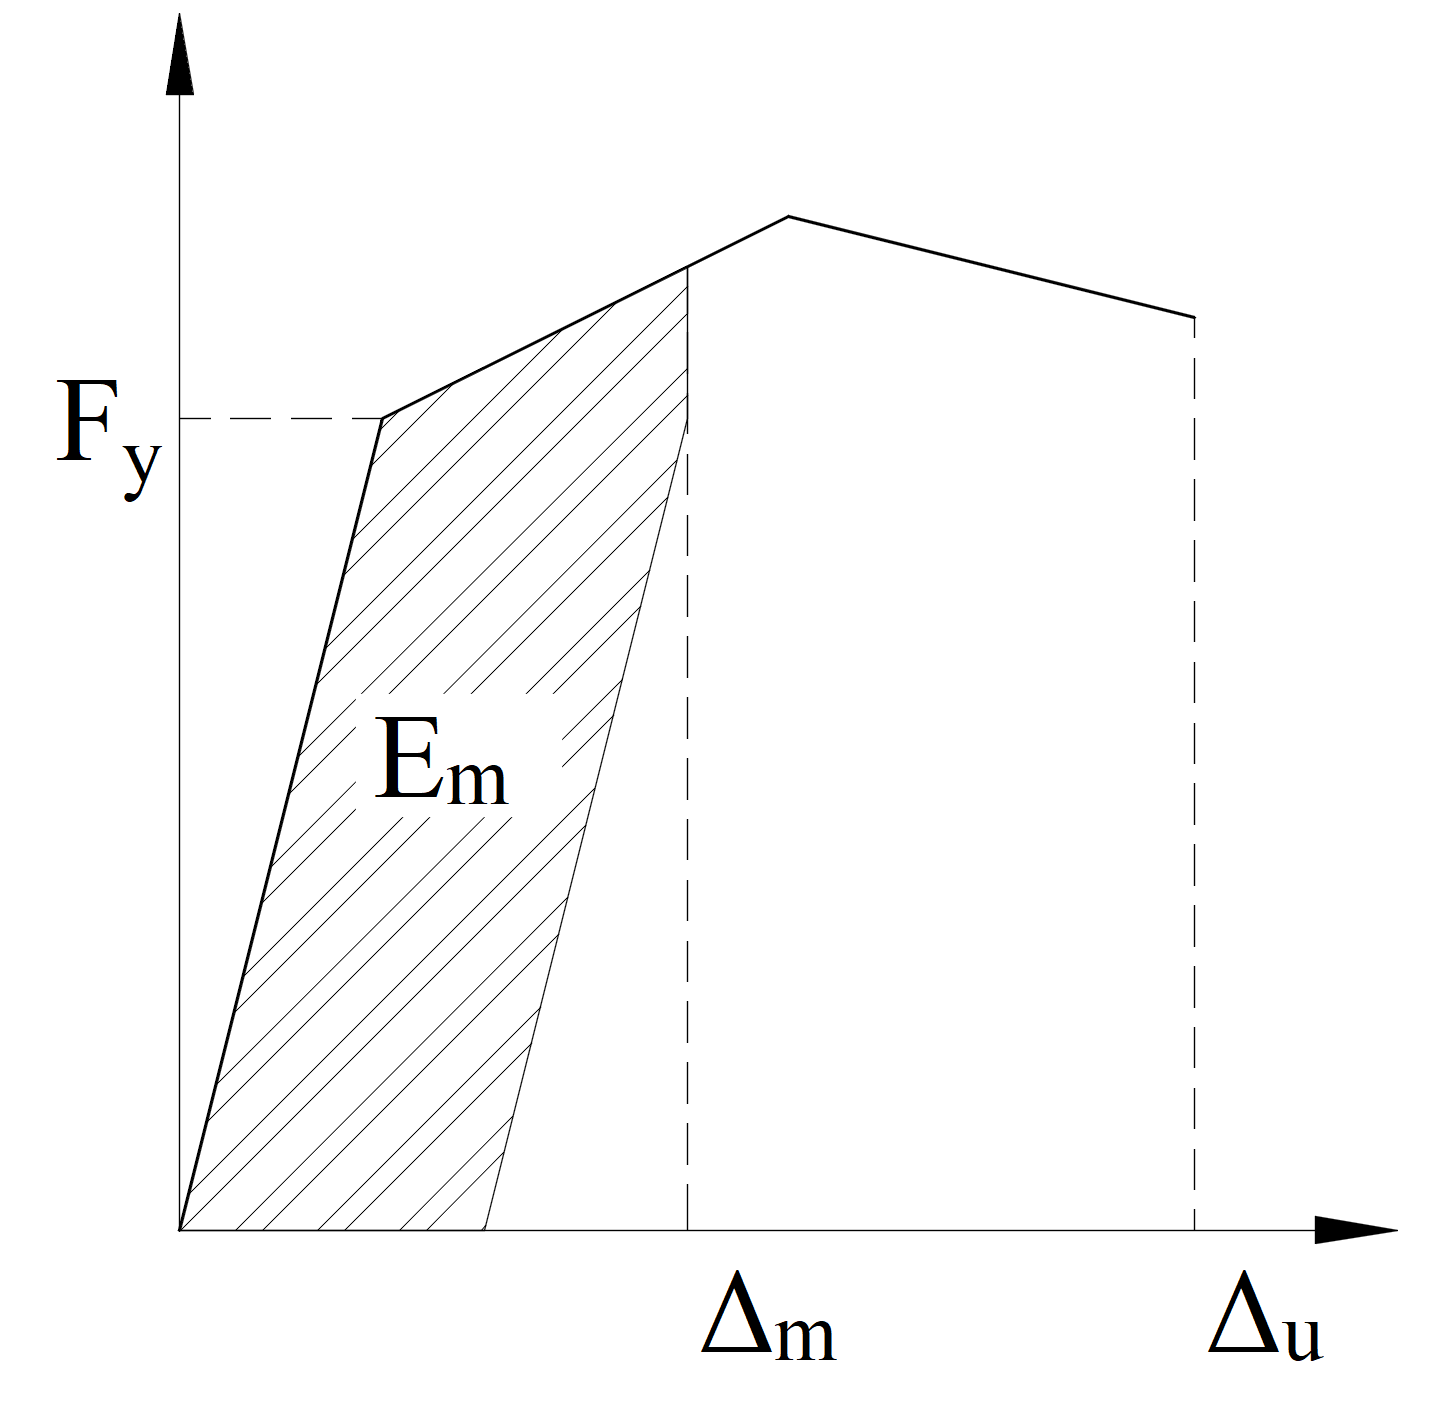
\includegraphics[width=0.9\textwidth]{Chapter-2/figs/Park_and_Ang_Model}
\caption{Parkn and Ang conceptual scheme}
\label{fig:Paa}
\end{figure}

This equation was derived for concrete elements. The first term here is a simple, pseudo-static displacement measure. It takes no account of cumulative damage, which is accounted for solely by the energy term. A figure on the concept is shown in \fref{fig:Paa}. The advantages of this model are its simplicity, and the flexibility on adpating the model to correlate with experimental data.  

In its current form, this model has several limitations. Firstly the calibration of the $\beta$ coefficient with observed damage, has shown to be very low ($\beta=0.05-0.15$) rendering the second term relatively inconsequential compared to the contribution of the first term. In addition, the model was derived for reinforced concrete with poor shear detailing. The correlations observed in this model also showed the data to be sparse. 

Depite its limitation, several studies have used or modified this model to study the effects of cumulative damage for different structures,  of relevant importance are those performed by \cite{Kunnath1992}, who used a modified Park and Ang model, to model damagae at the local level for elements in a structural analysis program IDARC 3.0, in this software for the case of multiple degrees of freedom buildings they also added parameters to consider the damage at the inter-story level and the global model. Ghosh et al \cite{Ghosh2015} developed a damage accumulation framework to develop probabilistic estimates of exceeding a damage index for multiple ground motions. Other regressions have been proposed by \cite{Khashaee}, {Fajfar1992}, {Roufaiel} but show no improvement in assessing the damage state of a structure. While these studies provide insight into some of the characteristics of damage accumulation they rely on the Park and Ang model and therefore carry the limitations of the model.

Krawinkler (1987) \cite{Krawinkler1987} proposed a method that would consider damage as a function of low cycle fatigue parameters, the form of this damage index for Steel Component, Weldements and local buckling have a general shape of the Miner model. This model relies on the accumulation of plastic deformations. While this model has proven to work well for the evaluation of individual elements it does not provide a way to generalize damage for other types of structures.

\subsection{Probabilistic Approach}

Increasing interest on the effect of cumulative damage has been experienced over recent years. These studies have focused on determining what is the increase in the risk of a structure due to the accumulation of factors due to many reasons such as multiple earthquakes, corrosion and life span of the structure. Two main approaches have been observed:

\begin{itemize}
	\item Probabilistic Framework
	\item Fragility Curves
\end{itemize}

Proababilistic network

One of the most widely used probabilistic network is the Pacific Earthquake Engineering Research Center (PEER) Performance Based Design. PEER PBD can be expressed by the following equation:
\begin{equation}
\nu_{DM}(dm^{LS})=\iint D_{DM|EDP}(dm|edp)|,dG_{EDP|IM}(edp|im)||\,d\nu_{IM}(im)|
\end{equation}

Mackie et al \cite{Mackie2007} on the basis of the PEER PBD developed the Performance Based Damage Design (PBDD) and Perfomance Based Loss Design (PBLD) by defining the probabilistic demand, damage, and loss model parameters in terms of reinforced concrete column damage. The RC column damage was defined on terms of drift ratios defined for the limit states of concrete spalling, bar buckling and failure. 

The authors show that for a given intensity measure (IM) and a confidence level of achieving a limit state, its is possible then to define the probability  of exceeding that limit state.

While this methodology was able to define damage and incorporate it into the PEER PBD framework, the authors did not consider a better way to establish a limit state such as strains. Also recent research has shown that other intensity measures such as spectral displacement at effective fir mode period provide a better intensity measure.


Fragility Curves

Another common trend in this subject is the use of fragility curves to estimate the effect of damage in structures. Two main approaches were found one of them relied on the Park and Ang Model Damage Index to define damage. The second approach relates damage to drift.

%Mention the three papers from Jaime Padget

While these studies provide a general view on how damage increases the likelihood of observing damage the methods used to arrive to those conclusions can be misleading since the definition of damage as either a Damage Index or Drift does not necessarily represent a quantifiable measure of damage it is our belief that strain based limit states will provide a better understanding and implications on the damage accumulation.